%%%%%%%% ICML 2021 EXAMPLE LATEX SUBMISSION FILE %%%%%%%%%%%%%%%%%

\documentclass{article}

% Recommended, but optional, packages for figures and better typesetting:
\usepackage{microtype}
\usepackage{graphicx}
\usepackage{subfigure}
\usepackage{booktabs} % for professional tables

% hyperref makes hyperlinks in the resulting PDF.
% If your build breaks (sometimes temporarily if a hyperlink spans a page)
% please comment out the following usepackage line and replace
% \usepackage{icml2021} with \usepackage[nohyperref]{icml2021} above.
\usepackage{hyperref}

% Attempt to make hyperref and algorithmic work together better:
\newcommand{\theHalgorithm}{\arabic{algorithm}}

% Use the following line for the initial blind version submitted for review:
\usepackage[accepted]{icml2021}
\usepackage{amsmath}
\usepackage{amssymb}
\usepackage{stmaryrd}

% If accepted, instead use the following line for the camera-ready submission:
%\usepackage[accepted]{icml2021}

% The \icmltitle you define below is probably too long as a header.
% Therefore, a short form for the running title is supplied here:
\icmltitlerunning{Reinforcement Learning 2023 Assignment 2}

\begin{document}

\twocolumn[
\icmltitle{Reinforcement Learning 2023, Master CS, Leiden University \\
   Assignment 2 on Deep Q Learning (DQN)}



% It is OKAY to include author information, even for blind
% submissions: the style file will automatically remove it for you
% unless you've provided the [accepted] option to the icml2021
% package.

% List of affiliations: The first argument should be a (short)
% identifier you will use later to specify author affiliations
% Academic affiliations should list Department, University, City, Region, Country
% Industry affiliations should list Company, City, Region, Country

% You can specify symbols, otherwise they are numbered in order.
% Ideally, you should not use this facility. Affiliations will be numbered
% in order of appearance and this is the preferred way.
\icmlsetsymbol{equal}{*}


\begin{icmlauthorlist}
\icmlauthor{Tom Stein (s3780120)}{lu}
\icmlauthor{Andrija Kuzmanov (s3766780)}{lu}
\icmlauthor{Tommaso Ancilli (s3674657)}{lu}
\end{icmlauthorlist}
   
\icmlaffiliation{lu}{Faculty of Science, Leiden University, Leiden, The Netherlands}

\icmlcorrespondingauthor{Tom Stein}{tom.stein@tu-dortmund.de}
\icmlcorrespondingauthor{Andrija Kuzmanov}{andrija.kuzmanov@gmail.com}
\icmlcorrespondingauthor{Tommaso Ancilli}{tommaso.ancilli@student.unisi.it}

% You may provide any keywords that you
% find helpful for describing your paper; these are used to populate
% the "keywords" metadata in the PDF but will not be shown in the document
\icmlkeywords{Reinforcement Learning, Machine Learning}

\vskip 0.3in
]

% this must go after the closing bracket ] following \twocolumn[ ...

% This command actually creates the footnote in the first column
% listing the affiliations and the copyright notice.
% The command takes one argument, which is text to display at the start of the footnote.
% The \icmlEqualContribution command is standard text for equal contribution.
% Remove it (just {}) if you do not need this facility.

%\printAffiliationsAndNotice{}  % leave blank if no need to mention equal contribution
\printAffiliationsAndNotice{\icmlEqualContribution} % otherwise use the standard text.

\begin{abstract}
This assignment report focuses on Deep Q Learning (DQN)
with an application to the CartPole environment. 
The basic concept of DQN is introduced along with the experience replay 
and target network improvements.
The effect of individual hyperparameters is studied empirically 
and through a hyperparameter scan.
A high degree of instability in the training process was observed, 
which is, to some extent, mitigated by specific adjustments of the parameters.
\end{abstract}

\section{Introduction}
\label{sec:introduction}
In this assignment, an agent has to learn how to balance a pole in the vertical position.
The environment presented is a well known and well-defined physical problem, being a reverse pendulum attached to a carriage through a joint.
The goal of this learning task is to keep the pole in place while moving the cart left or right.
The possible action space is made up by a set of only two possible movements ${0,1}$, where $0$: the cart is pushed to the left; $1$: the cart is pushed to the right.
The state space is composed of four values: position and velocity of the cart, angle and angular velocity of the pendulum.
The agent receives a reward of $+1$ for every action performed that results in keeping the pole in an upright state ($\pm 12^\circ$).
The environment is reset to the initial condition every time that the value of the angle between the pole and the vertical line is bigger than $12^\circ$ or when the cart leaves the range horizontal range $(-2.4;2.4)$.
The maximum reward in the environment is limited to 500 because there is no natural end to the balancing problem, and obtaining a reward of 500 demonstrates the ability to balance the pole quite well.

The old paradigm, where all the q-values could be stored in a table and updated directly to determine the optimal policy, is not suitable anymore.
The reason lies in the exponential amount of memory required to store all the possible states (curse of dimensionality).
Given the impossibility of memorizing all the possible states, the agent has to learn how to generalize to unseen data.
This can be done through the application of deep learning.
It is known that an Artificial Neural Network has the property to approximate any function~\cite{Cybenko}, enabling the possibility of inferring an unseen state and having a more compact representation of the solution itself.
The resulting algorithm, generated by the union of Deep learning and Q-learning, is called Deep Q-Network algorithm (DQN).
In this report, the neural network has to approximate the Q-values using a parameterized function.
This approach is also called value-based.

\begin{equation}
    Q_{\theta} :  s \rightarrow q
    \label{eq:value-based-approach}
\end{equation}
where, $s \in S$ where $S$ represents the set of all the possible states and $q$ is the Q-values of the admissible actions.


The remaining chapters are structured as follows.
In \autoref{sec:methodology}, the underlying theories regarding the separate approaches will be shown.
The \autoref{sec:results} is dedicated to the discussion of the optimal configuration for the hyperparameters tuned on the DQN architecture, which exploits the advantages of replay buffer and target network.
In this portion of the report the parameters are tweaked individually, which places this unit at the opposite end of the \autoref{sec:bonus}.
Thereupon, this section is dedicated to study the relationship that each hyperparameter has with the others.
Finally, in \autoref{sec:discussion} the results are summarized and insights into what could have been improved are given.
As a baseline comparison to juxtapose to the different solution will be the random one.
In this one, the agent performs random moves, and the average cumulative reward is set to $22.4$.

\section{Methodology}
\label{sec:methodology}
This section will examine methods used to solve the cart pole balancing problem.
Ideally, the problem would be solved with the Q-learning method, since it is easy to implement and interpret.
However, due to continuous state space it is not possible to store a $Q(s,a)$ value for every state-action pair.
Because of that, the deep learning methods will be used to estimate the $Q(s,a)$ value for any given state-action pair.
Firstly, the DQN or Deep Q-learning method will be examined.
Secondly, the DQN method will be improved with experience replay and a target network.

\subsection{DQN}
\label{subsec:dqn}
DQN is one of the most known deep reinforcement learning algorithms.
It is based on the tabular Q-learning method, but instead of obtaining the $Q$ value from a table,
a neural network is trained (the parameters are adjusted) to predict the values given a certain state.
A neural network is a machine learning structure that contains a large amount of parameters that can be tuned
to represent a certain function.
The DQN agent learns by taking steps in the environment and updating the $Q$ value estimates by using the obtained reward.
The update process is called bootstrapping, as it refines the old estimates using new updates~\cite{DBLP:books/sp/Plaat22}.
In order to update the current $Q(s,a)$ value, first a step is taken, reward is obtained, and the (expected)
target value $GT$ of $Q(s,a)$ is computed with the following equation:

\begin{align}
   \label{eq:calculating-target}
    GT = r + \gamma \cdot \max_{a^\prime} Q_{\theta}(s^\prime, a^\prime)
\end{align}

From \autoref{eq:calculating-target} it can be seen that the target is based on the received reward and the discounted
value of the next state.
The letter $\gamma$ represents the discount factor and the letter $\theta$ represents the parameters of the neural network $Q$.
The target and our current $Q(s,a)$ estimate can then be used to compute the loss using a pre-defined loss function.
A loss function can be any mathematical function that measures the difference between the predicted output and the
actual output.
One of the most common examples when it comes to regression problems is the mean squared error function displayed
in \autoref{eq:mse}, 
where $x$ and $y$ denote the predicted and the actual values, while $n$ denotes the number of values.

\begin{align}
   \label{eq:mse}
   \alpha(x, y) = \frac{1}{n} \cdot \sum_{i = 0}^{n} [(x_i - y_i)^2]
\end{align}

Using the computed loss, the parameters $\theta$ can be optimized in order to minimize the loss.
One of the most common algorithms for optimization is called stochastic gradient descent (SDG).
It computes the gradient of the loss function with respect to the parameters $\theta$.
The gradients are then used to push each of the parameters in the opposite direction of the gradient and with that minimize
the loss.
The amount by which each of the parameters is pushed is determined by the learning rate $\alpha$.
The smaller the $\alpha$ the smaller the step taken in the opposite direction of the gradient.
In the experiments conducted in this report, the Adam optimizer is used, which tries to improve upon the SDG optimizer
by using the first and the second moments of the gradient to adapt the learning rate for each weight
of the neural network~\cite{kingma2014adam}.

The algorithm~\ref{alg:dqn} displays how a DQN algorithm learns.
Similar to regular Q learning, there are two loops.
The first loop defines the amount of the episodes that need to be executed, and the second loop executes
the episode until termination.
While performing an episode, first an action must be picked based on the $Q$ value estimates,
that are obtained by passing the current state $s$ to the neural network.
Because of this, the estimates will be completely random in the beginning, but will improve as more moves are made and learned.
Different policies for action-selection can also be used, for example, epsilon-greedy or the Boltzmann policy
whose parameters can be tuned to incorporate a balance between exploration and exploitation.

After obtaining an action, it can then be executed inside the environment in order to obtain the next state $s^\prime$
as well as the reward $r$ for performing that action.
Afterwards, the $Q(s,a)$ value and the target estimate can be computed (using \autoref{eq:calculating-target}).
The loss is equal to the squared difference between the target $Q$ value and the $Q(s,a)$ value that was computed.

Once terminal state is reached, the gradient of the loss function with respect to the neural network's parameters is calculated.
Those gradients are then provided to the backward pass function that optimizes the parameters.


\begin{algorithm}
   \caption{DQN pseudocode}
   \begin{algorithmic}
      \REQUIRE environment, Qnet, $\alpha \in (0,1]$, $\gamma \in [0,1]$, $\epsilon \in [0,1]$, max\_epoch $\in$ $\mathbf{N}$
      \STATE $s = s_0$ \COMMENT{Initialize start state}
      \FOR{i = 0..max\_epoch}
         \STATE sum\_sq = 0
         \WHILE{$s$ not TERMINAL}
            \STATE $a$ = select\_action(Qnet(s))
            \STATE $s^\prime$, $r$ = env.step($a$)
            \STATE output = max(Qnet($s$))
            \STATE target = $r$ + $\gamma \cdot$ max(Qnet($s^\prime$))
            \STATE sum\_sq += $(target - output)^2$
            \STATE $s = s^\prime$
         \ENDWHILE
         \STATE grad = Qnet.gradient(sum\_sq)
         \STATE Qnet.backward\_pass(grad, $\alpha$)
      \ENDFOR
      \STATE \textbf{Return:} Qnet
   \end{algorithmic}
   \label{alg:dqn}
\end{algorithm}

While the algorithm seems promising, it still faces three important challenges.
Firstly, the convergence of the algorithm depends on the full coverage of the state space, which in the case of the described
problem is just not feasible.
Secondly, there is a strong correlation between subsequent training samples that can lead to poor generalization and overfitting.
Thirdly, a bootstrapped target is used to calculate the loss of each prediction.
The weights of the network that predicts the target change after every optimization step, which can lead to unstable learning~\cite{DBLP:books/sp/Plaat22}.

The problems posed in the previous paragraph can not be fully solved, but it is possible to minimize their impact.
Firstly, the problem of low coverage can be improved by setting a high probability of taking an exploratory step.
The higher the probability, the higher amount of state space the algorithm will explore.
Secondly, the high correlation problem can be improved by implementing a replay buffer, which is described in \autoref{subsec:experience-replay}.
Thirdly, a secondary neural network that is updated less frequently can be implemented and used only for target predictions.
This approach is called target network and is explained in \autoref{subsec:target-network}
Finally, the learning can be stabilized by setting a very low learning rate $\alpha$ that will minimize the change between
subsequent target predictions.

\subsection{Experience Replay}
\label{subsec:experience-replay}

Plain DQN algorithm suffers from high correlation between subsequent states.
This means that the agent frequently visits same states and makes similar actions,
and consequently trains the neural network on very similar samples.
What is more, because of bootstrapping and function approximation the algorithm can forget some useful behaviour that it learned in the past.
This can lead to overfitting, instability in the training process, and consequently poor generalization.
Moreover, it may also fail to cover a significant amount of state space and get stuck
in the local optima because of this.
To break the correlation, a replay buffer, a buffer that stores experiences, can be used.
Using this, the DQN agent no longer needs to learn from subsequent experiences, as it can obtain random samples
from the replay buffer and learn from them instead.
Breaking the correlation between subsequent samples improves coverage and generalization of the algorithm~\cite{DBLP:books/sp/Plaat22}.
Without this, DQN can become biased towards the most recent experiences and forget the previous experiences
that are still very relevant for the task.

\subsection{Target Network}
\label{subsec:target-network}

In order to improve the stability of learning and reduce the divergence cause by frequent weight updates,
a target network can be introduced~\cite{DBLP:books/sp/Plaat22}.
Target network $\hat Q$ is a new neural network that the algorithm will use to output the target values.
The newly added network is structurally a copy of the value network $Q$, but it gets updated every $n$ steps
by copying the parameters of the neural network $Q$ that is used for action selection ($\hat Q = Q$).
That way the target predictions remain stable for a longer period of time.
To calculate the target value, the \autoref{eq:calculating-target} can still be used, however, instead of using the $Q_\theta$
neural network it needs to bo replaced with $Q_{\theta - i}$ neural network where $\theta - i$ stands for the parameters
which were used $i$ steps ago.
In this case variable $i$ stands for the number of time steps since the target neural network $\hat Q$ was last updated.
After every $n$ steps, the $\hat Q_{\theta - i}$ is updated, making the variable $i$ equal to 0 and $\hat Q_{\theta - i}$
equal to $Q_\theta$.

\section{Results}
\label{sec:results}
In this section, we will present the results obtained by tuning the individual hyperparameters. 
In order to have a common baseline for making comparisons, we have collected the baseline that will be used in the \autoref{baseline_config}. 
The values used to fill in \autoref{baseline_config} were an educated guess, stemming from previous runs.\\
Aware of the fact that the data we are going to present need statistical significance, 
otherwise it would be impossible to draw valid conclusions, we decided to use 5 as the number of repetitions as in our opinion, 
it presented a fair compromise between statistical significance and the computational power required to perform the calculations.\\
As previously mentioned in \autoref{introduction}, we have taken as a reference an agent that performs causal sequences. 
The architecture of this agent is rather elementary, containing only the initial and final layers. 
The average number of random moves performed before the environment is reset was found as the average of the total rewards for each episode.\\ 

\begin{table}[t]
   \caption{Baseline hyper-parameters config}
   \label{baseline_config}
   \vskip 0.15in
   \begin{center}
   \begin{small}
   \begin{sc}
   \begin{tabular}{lcccr}
   \toprule
   Parameter & Value \\
   \midrule
   Network Architecture    & $4-64-32-32-2$ \\
   Learning rate           & $0.001$ \\
   Learning rate decay     & $1.0$   \\
   Epochs                  & $1000$ \\
   Policy                  & epsilon greedy \\
   Initial epsilon         & $0.2$ \\
   Decay                   & $0.99$ \\
   Minimal epsilon value   & $0.01$ \\
   Gamma                   & $0.9$ \\
   Sampling rate           & $2$ \\
   Buffer size             & $1000000$ \\

   \bottomrule
   \end{tabular}
   \end{sc}
   \end{small}
   \end{center}
   \vskip -0.1in
   \end{table}

   Five different learning rates have been taken into account to detect the best one \autoref{comp_learning_rate}. 
   Beginning our consideration with the highest value, it can be clearly seen how this value is not suitable at all, 
   leading the agent to receive an average reward that does not even reach the threshold. 
   The learning rate has a value of $0.01$ but, despite being able to learn relatively quickly in the first hundreds of episodes, 
   the progression is not sustained in the remaining parts. 
   Indeed, after the cumulative reward peak has reached around the $190^{th}$ episode, the cumulative reward experiences oscillatory behavior, 
   varying within a range of $75$ and $30$ moves before the environment is set to the initial state.\\
   Having a look at the last three learning rates in \autoref{comp_learning_rate}, we can notice how close they are in terms of performances. 
   We have selected as the best learning rate the one with the value of $5$x$10^{-4}$. 
   The reasons for this choice lie in some considerations that can be drawn by looking at the plot.\\
   Firstly, if a comparison can be made between the learning rate with a value of $0.001$ and $5$x$10^{-4}$, the highest learning rate is thought to receive higher rewards in the first two hundred episodes. 
   However, letting the episodes go on, we can clearly see how $0.0005$ outperforms the other value.\\
   Secondly, our attention can be focused on the comparison between the two smallest learning rates. 
   In this case, the main reason why we have decided to prefer $5$x$10^{-4}$ over $1$x$10^{-4}$ is the standard error. 
   Although the smaller learning rate is more stable and less subjected to fluctuation during the training process, in accordance with the theory, 
   we can notice how its standard deviation is larger than $5$x$10^{-4}$, bringing to realization that this variability could affect the study in \autoref{sec:discussion}.

   \begin{figure}[ht!]
      \centering
      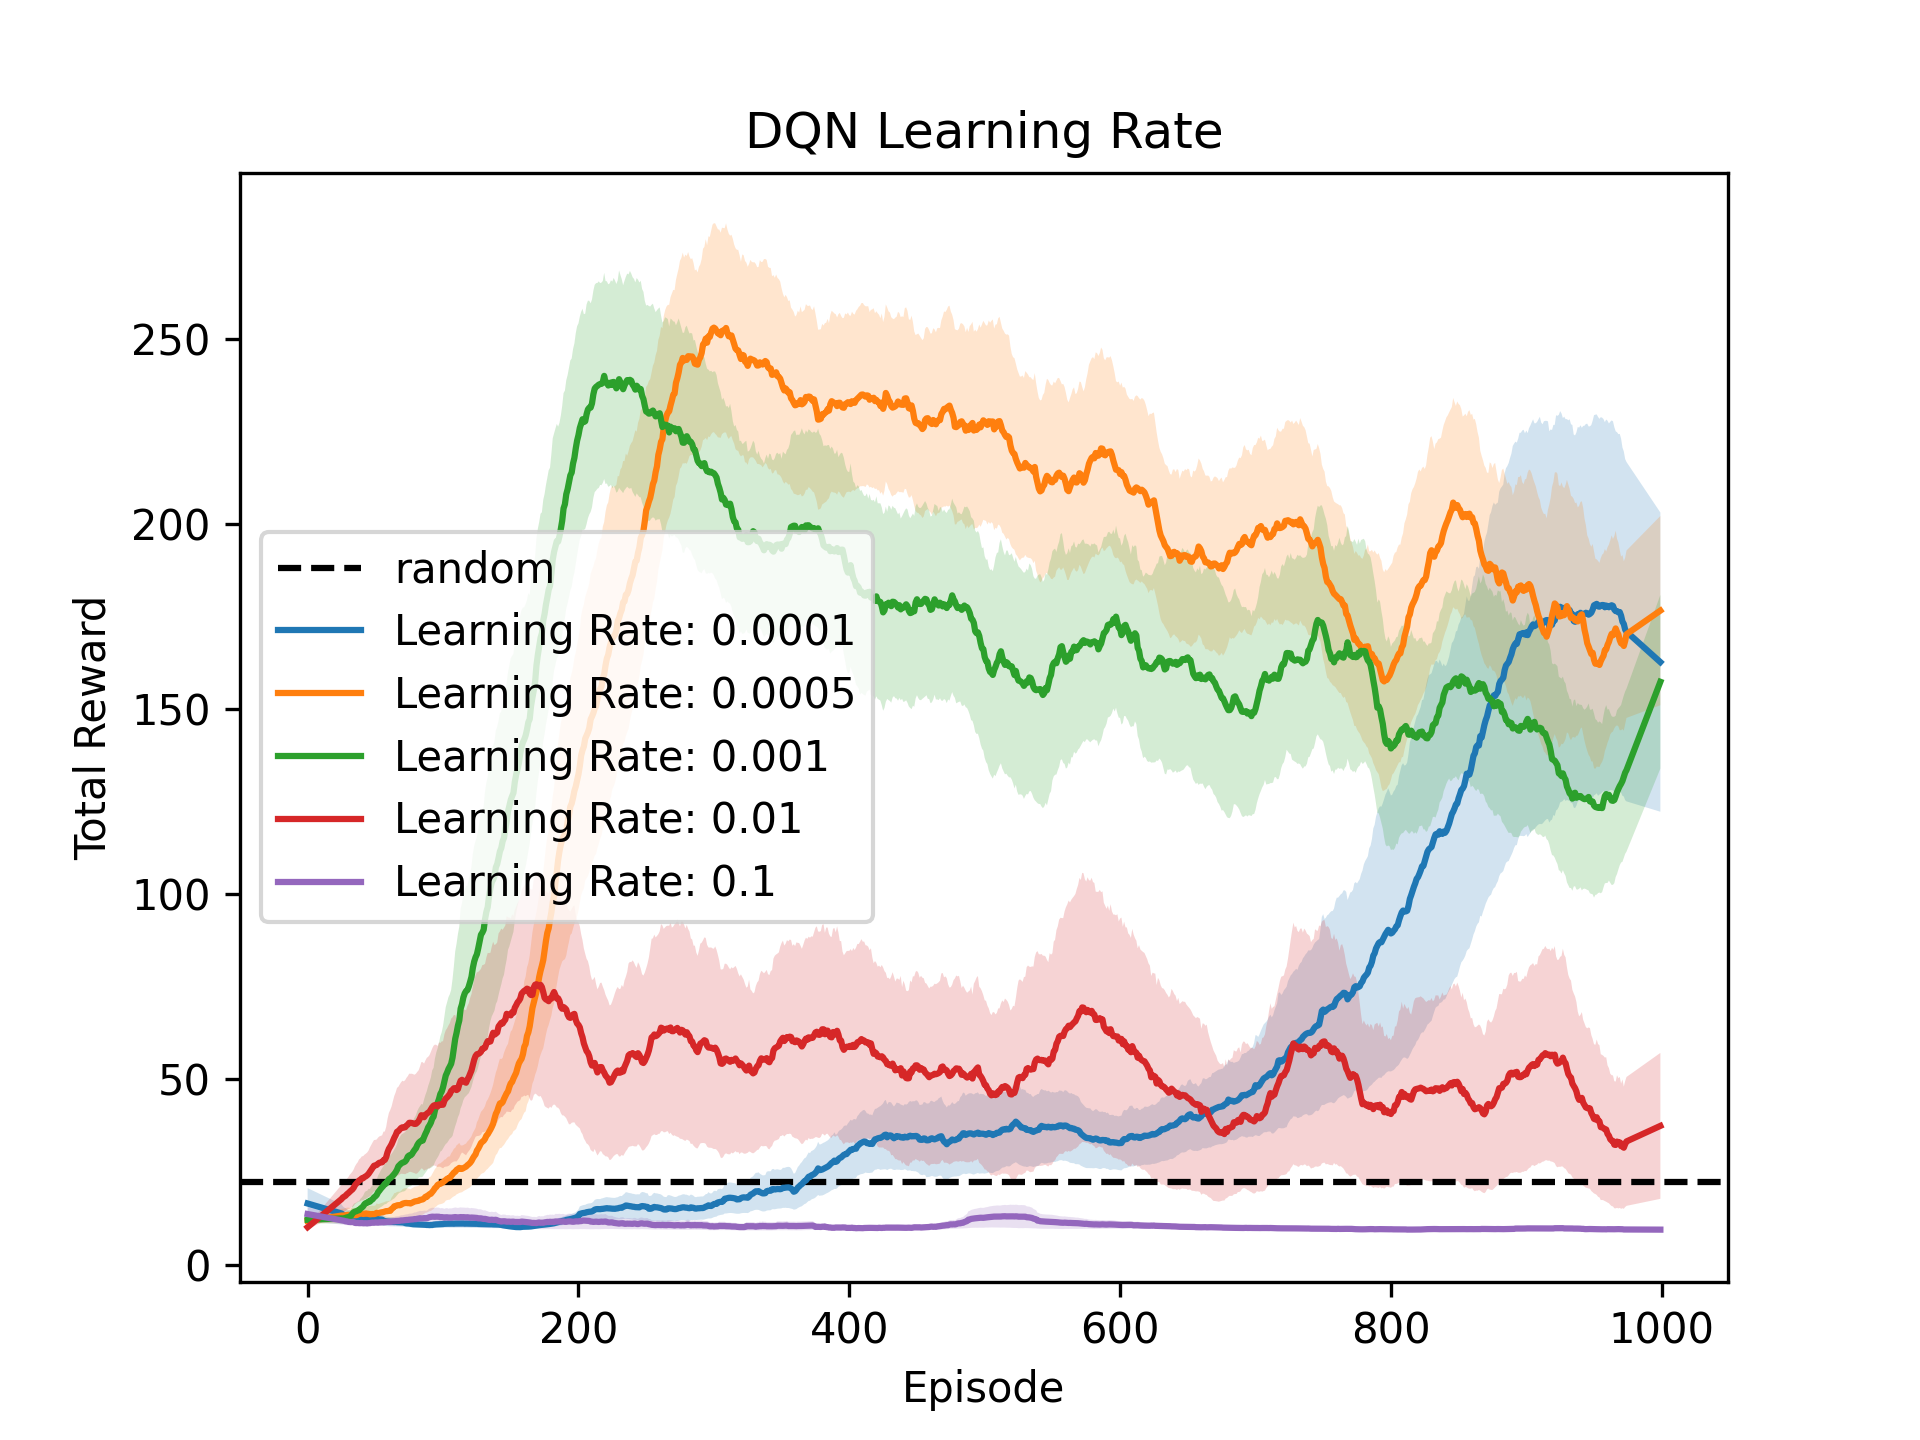
\includegraphics[width=\columnwidth]{assets/fig_hp/learning_rate.png}
      \caption{Comparison between five different learning rates. The think line represents the average performance, while the faided line is the standard deviation. 
      }
      \label{comp_learning_rate}
   \end{figure}
 
   Concerning the architecture for the neural network, we have decide to restrict our search guess into finding the best MLP (MultiLayer Perceptron) architecture.
   Five different architecture has been tested as the \autoref{comp_nn_arch} reports. 
   In each of the different architecture the number of hidden layers and neurons is chanching. 
   Giving a closer look at the results we can already discard two different architectures. 
   The architectures with the following structure $4-256-128-32-2$ and $4-32-128-256-2$ have closely related performances, for this reason the Occam's razor was used as a principle to discard them.\\
   For the same principle the architecture with $4-64-32-32-2$ is preferred over $4-32-64-64-2$. 
   
   I do not know what to write honestly, so i give two different versions and we select the best one:\\

   We have decided to adopt the architecture $4-128-128-2$ over $4-64-32-32-2$ because of its total reward reached at the end of the training. 
   In particular, although the tuning of the parameters was arduous requiring almost $400$ episodes to reach the random threshold, 
   after that an constant growth has been recorded, and the data shows at the end of the training, the agent was able to keep the pole in the vertical position for more than 200 moves.\\
   We have decided to prefer the smaller one $4-64-32-32-2$ over the bigger one $4-128-128-2$ for the same thought that we have adopted in the previous steps. 
   Indeed, the smaller architecture has nearly a sixth of the parameters of the other, and surprisingly the performances are almost the same. 
   As a support of our reasoning, we can argue that the architecture with only two hidden layers is really unstable and thus it is reflected also on the standard deviation.
   

   \begin{figure}[ht!]
      \centering
      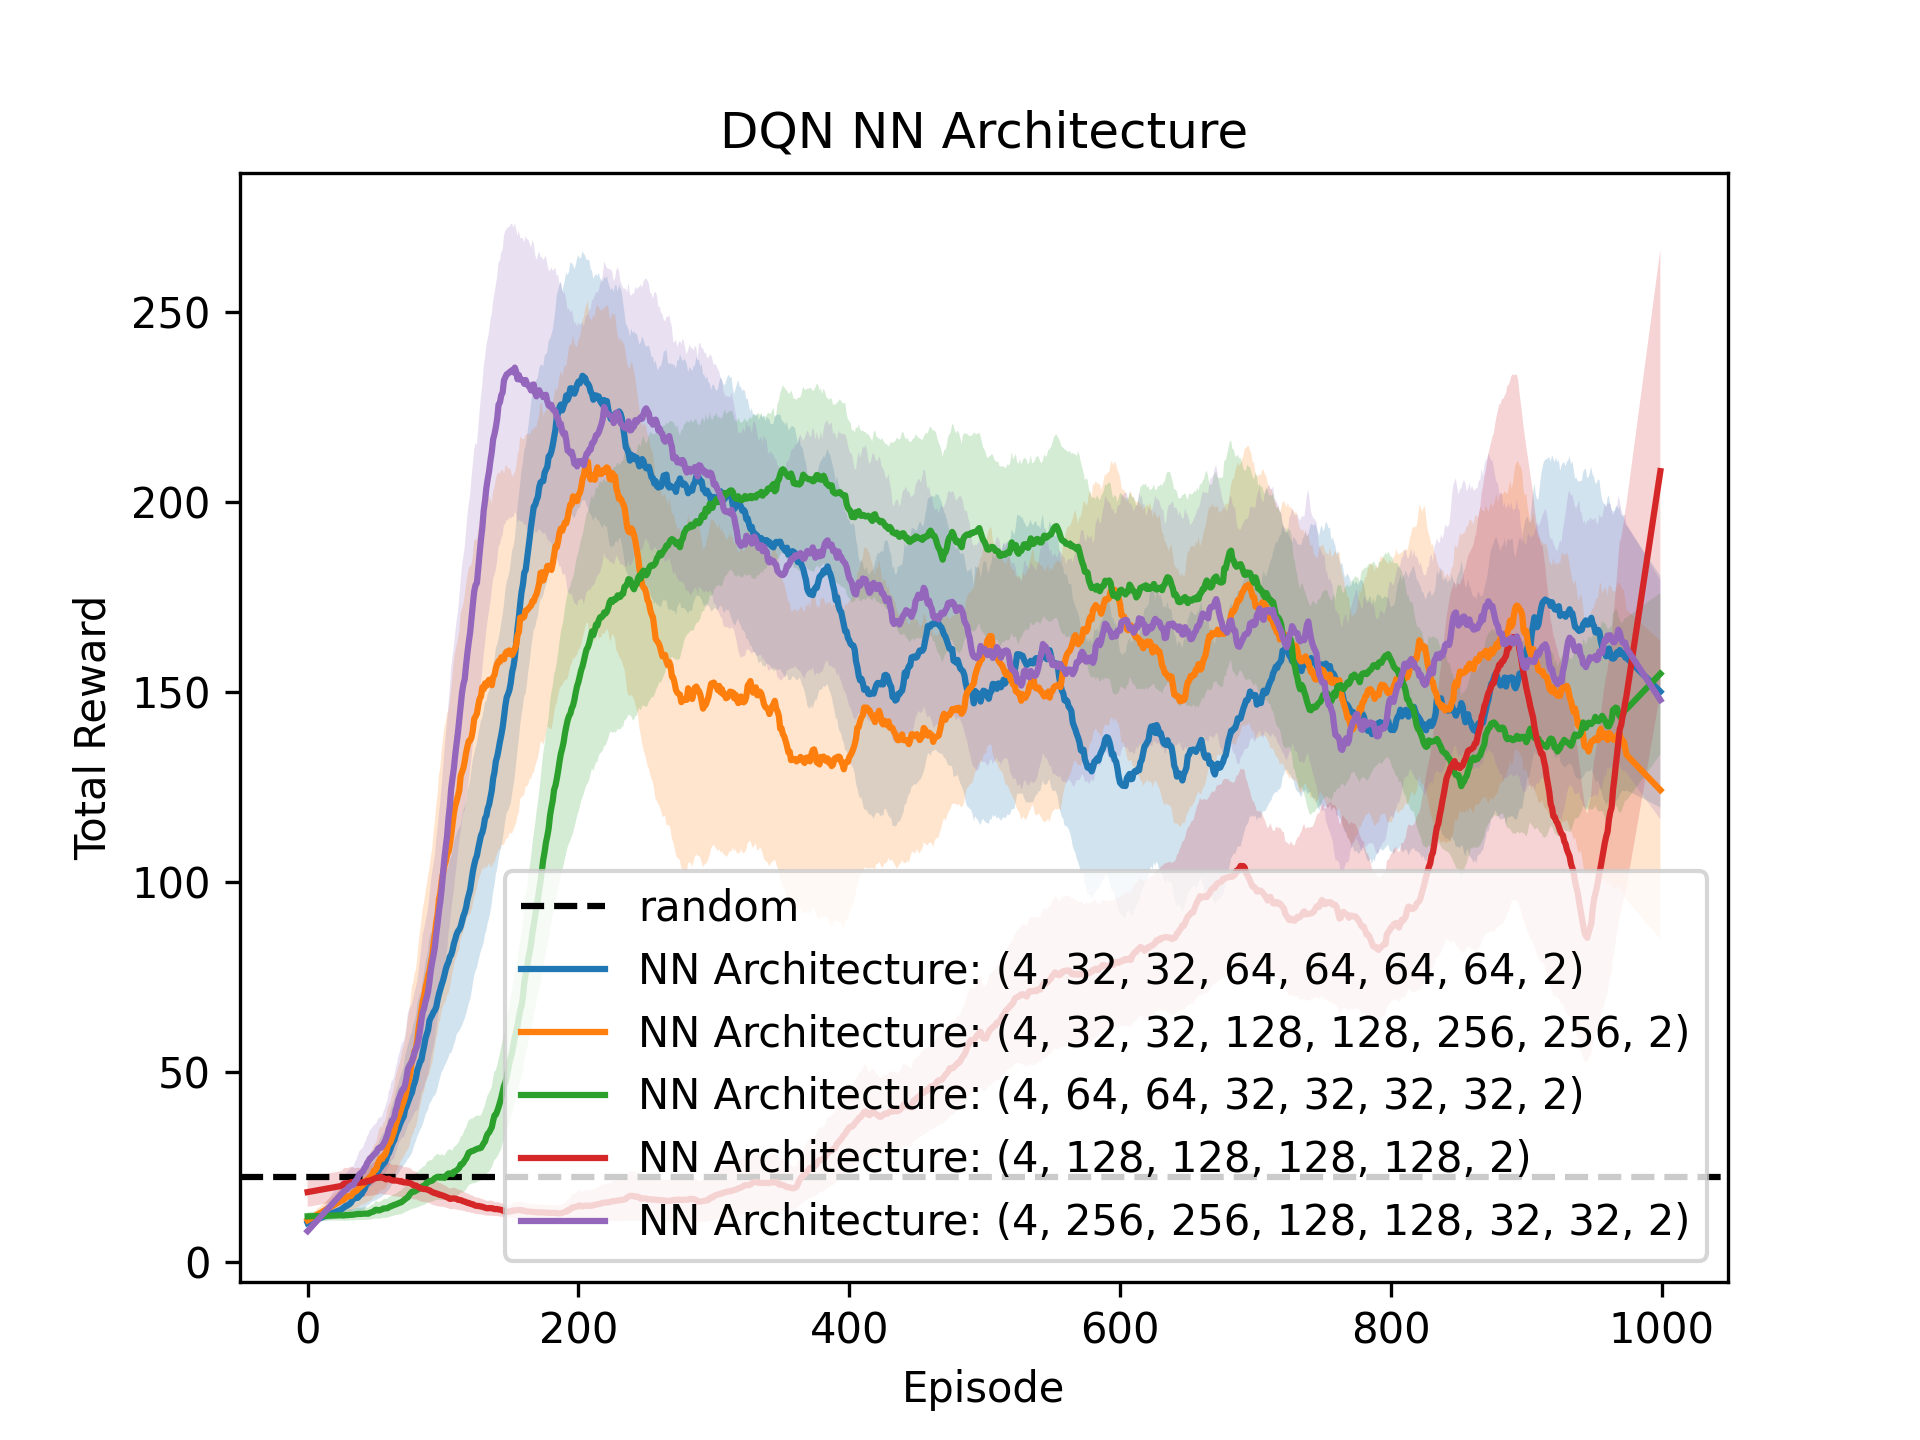
\includegraphics[width=\columnwidth]{assets/fig_hp/nn_architecture.png}
      \caption{Comparison between five different learning rates. The think line represents the average performance, while the faided line is the standard deviation. 
      }
      \label{comp_nn_arch}
   \end{figure}

% Explain methodology
%     Number of repetions was choosen as 5 as a trade-off between statistical significance and computation time
%     Choose of baseline parameters (our educated guesses from some prior runs)
%        - Epochs = 1000
%     Why parameters we varied and what ranges
%        - Buffer size in the range up to 500k (because that is the limit given by 1000 Epochs * 500 steps)

\subsection{DQN with ER and TN}
\label{subsec:dqn-with-er-and-tn}

% TODO: Mention catastropic forgetting

\subsection{DQN ablation study}
\label{subsec:dqn-ablation-study}

% Show what happens if we cut out parts of the model architecture.

\section{Discussion}
\label{sec:discussion}
% Discuss results in summary here


% Improvements
%   Use soft update from PolicyNet to Target net instead of hard copy every x epochs
%   Use early stopping to limit effect of overfitting and catastrophic forgetting and reduce computation time
%   Use other Optimizer (SGD) and loss metric (Huber-loss)

\section{Hyperparameter Scan - Bonus}
\label{sec:bonus}
In the \autoref{sec:results}, only individual hyperparameters were analyzed in isolation.
This approach does not take into account the dependencies between the different hyperparameters 
such as learning rate and batch size~\cite{DBLP:conf/iclr/SmithKYL18}.
For this reason, a comprehensive hyperparameter scan was performed, in which models were trained on random combinations of the hyperparameters. 
The definition of the hyperparameter space\footnote{\texttt{wandb\_sweep\_config.yaml}} 
intentionally does not make use of continuous value ranges like $[0.8, 1.0]$ but a preselection of discrete values to be able to group and plot the results more easily.
The hyperparameter space contains about 300 million combinations and is too large to be fully searched (i.e. grid search). 
Therefore, random search in combination with parallel experiments was used to search this large space in a reasonable time.
To support this, the platform Weights and Biases~\cite{wandb} was used to log all experiments and to orchestrate the hyperparameter scan across multiple computers.
The results are shown in \autoref{sec:hyperparameter-scan-results},
% TODO Update link to wandb
but can also be viewed interactively online\footnote{\url{https://api.wandb.ai/links/rl-leiden/udme67qe}}. 
In total 166 parameter combinations were evaluated in 6 days compute time.

The results again illustrate the instability caused by wrong parameter selection or catastrophic forgetting, 
since numerous runs only achieve poor results, much worse than a random agent. 
Apart from this, there are also three positive findings.
Firstly, the results of the hyperparameter scan, when considered in isolation, 
support the findings from \autoref{sec:results}. 
For example, a larger experience buffer size again shows a significant improvement in performance (see \autoref{fig_hyperparameter_scan_isolated_buffer_size}). 

% In the unusual situation where you want a paper to appear in the
% references without citing it in the main text, use \nocite
\nocite{DBLP:books/sp/Plaat22}

\bibliography{main}
\bibliographystyle{icml2021}


\appendix
\section{Hyperparameter Scan Results}
\label{sec:hyperparameter-scan-results}

% TODO Update image
\begin{figure*}[ht!]
   \centering
   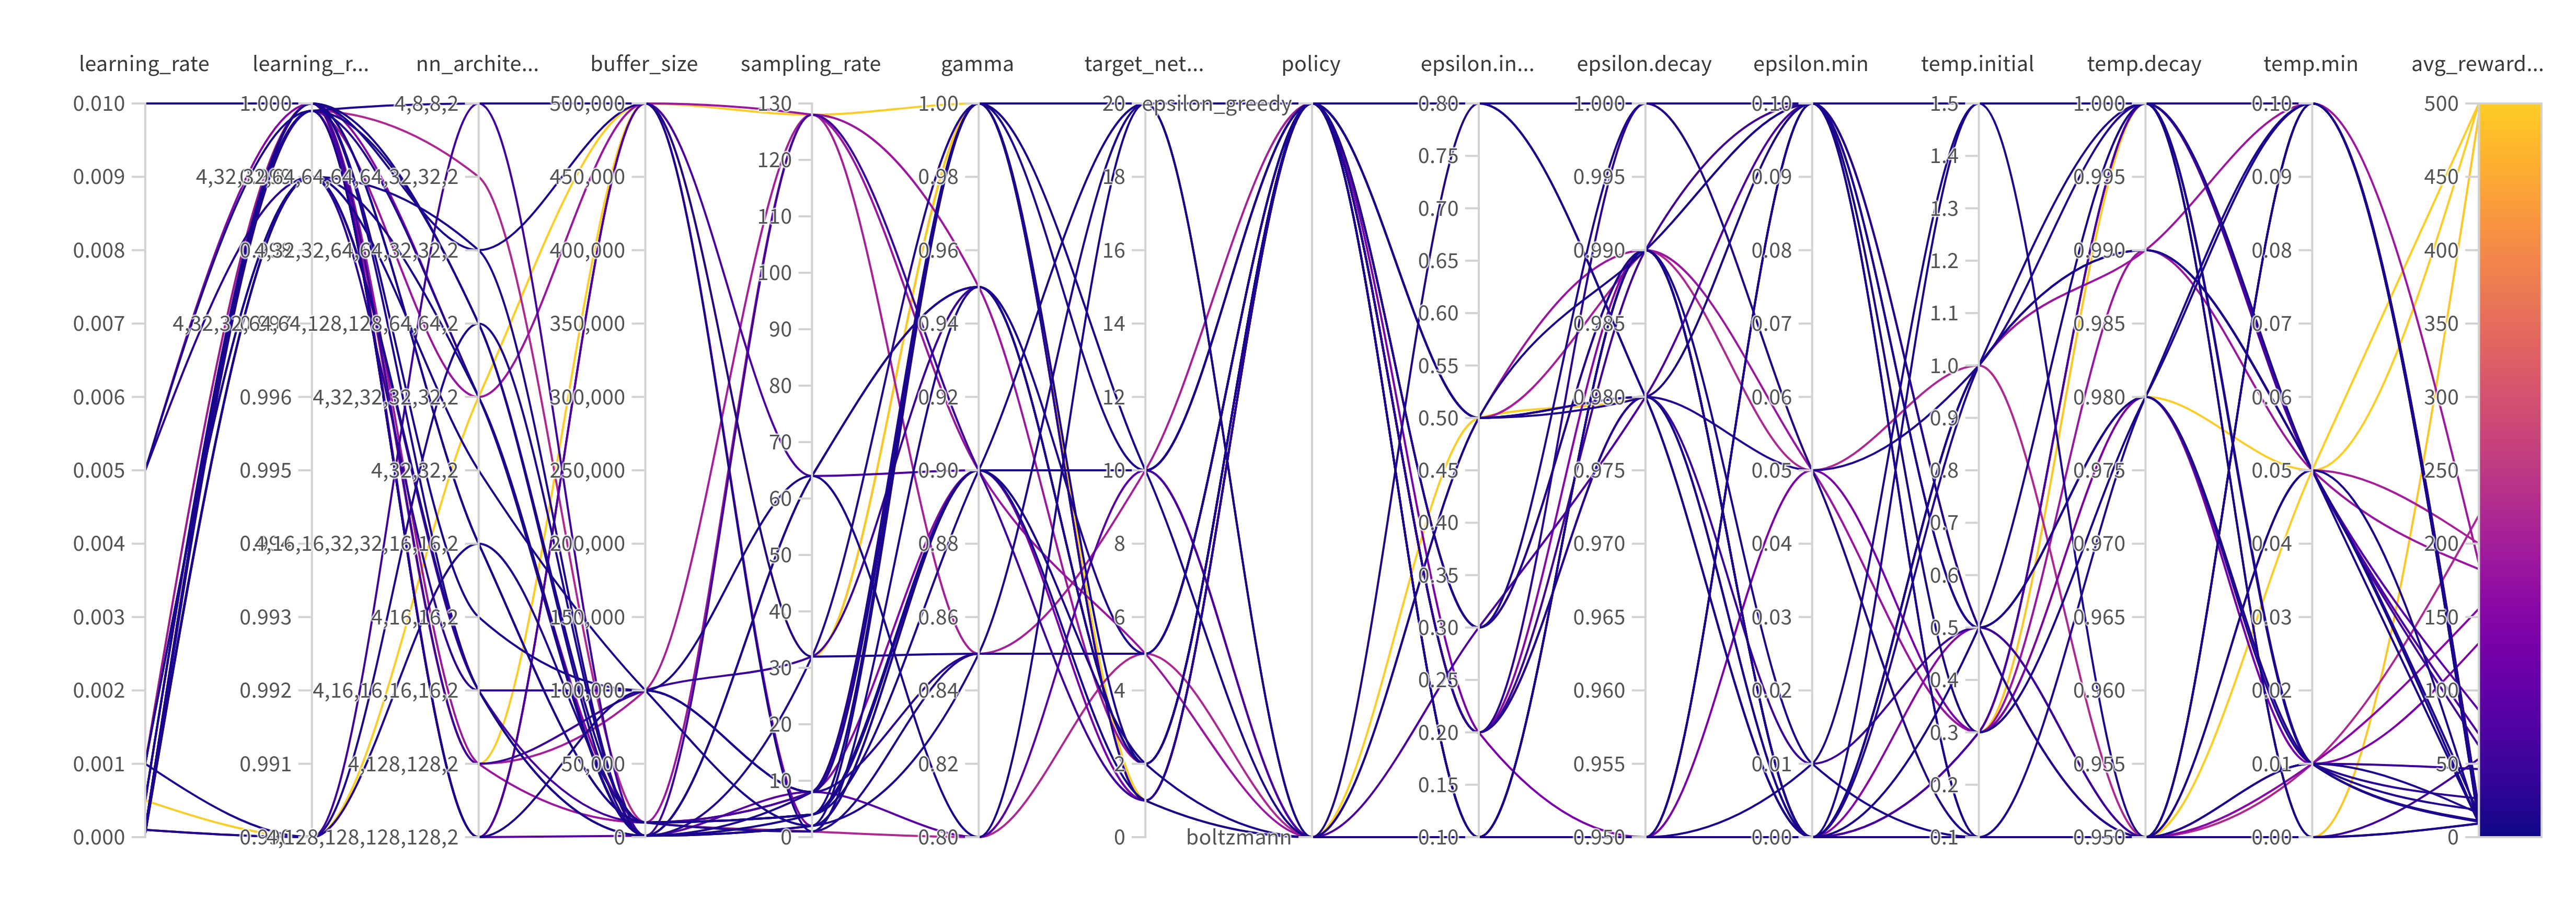
\includegraphics[width=\textwidth]{assets/hyperparamter-scan/W&B Chart 3_30_2023, 2 24 25 PM.png}
   \caption{Parallel axis plot of the hyperparameter scan. 
      Each line shows a single parameter configuration that was evaluated. 
      The color indicates the performance measured by the average of the last 100 epochs (see legend on the right). 
      Higher average reward (yellow) is better.
   }
   \label{fig_hyperparameter_scan_parallel_axis}
\end{figure*}


\begin{figure}[ht!]
   \centering
   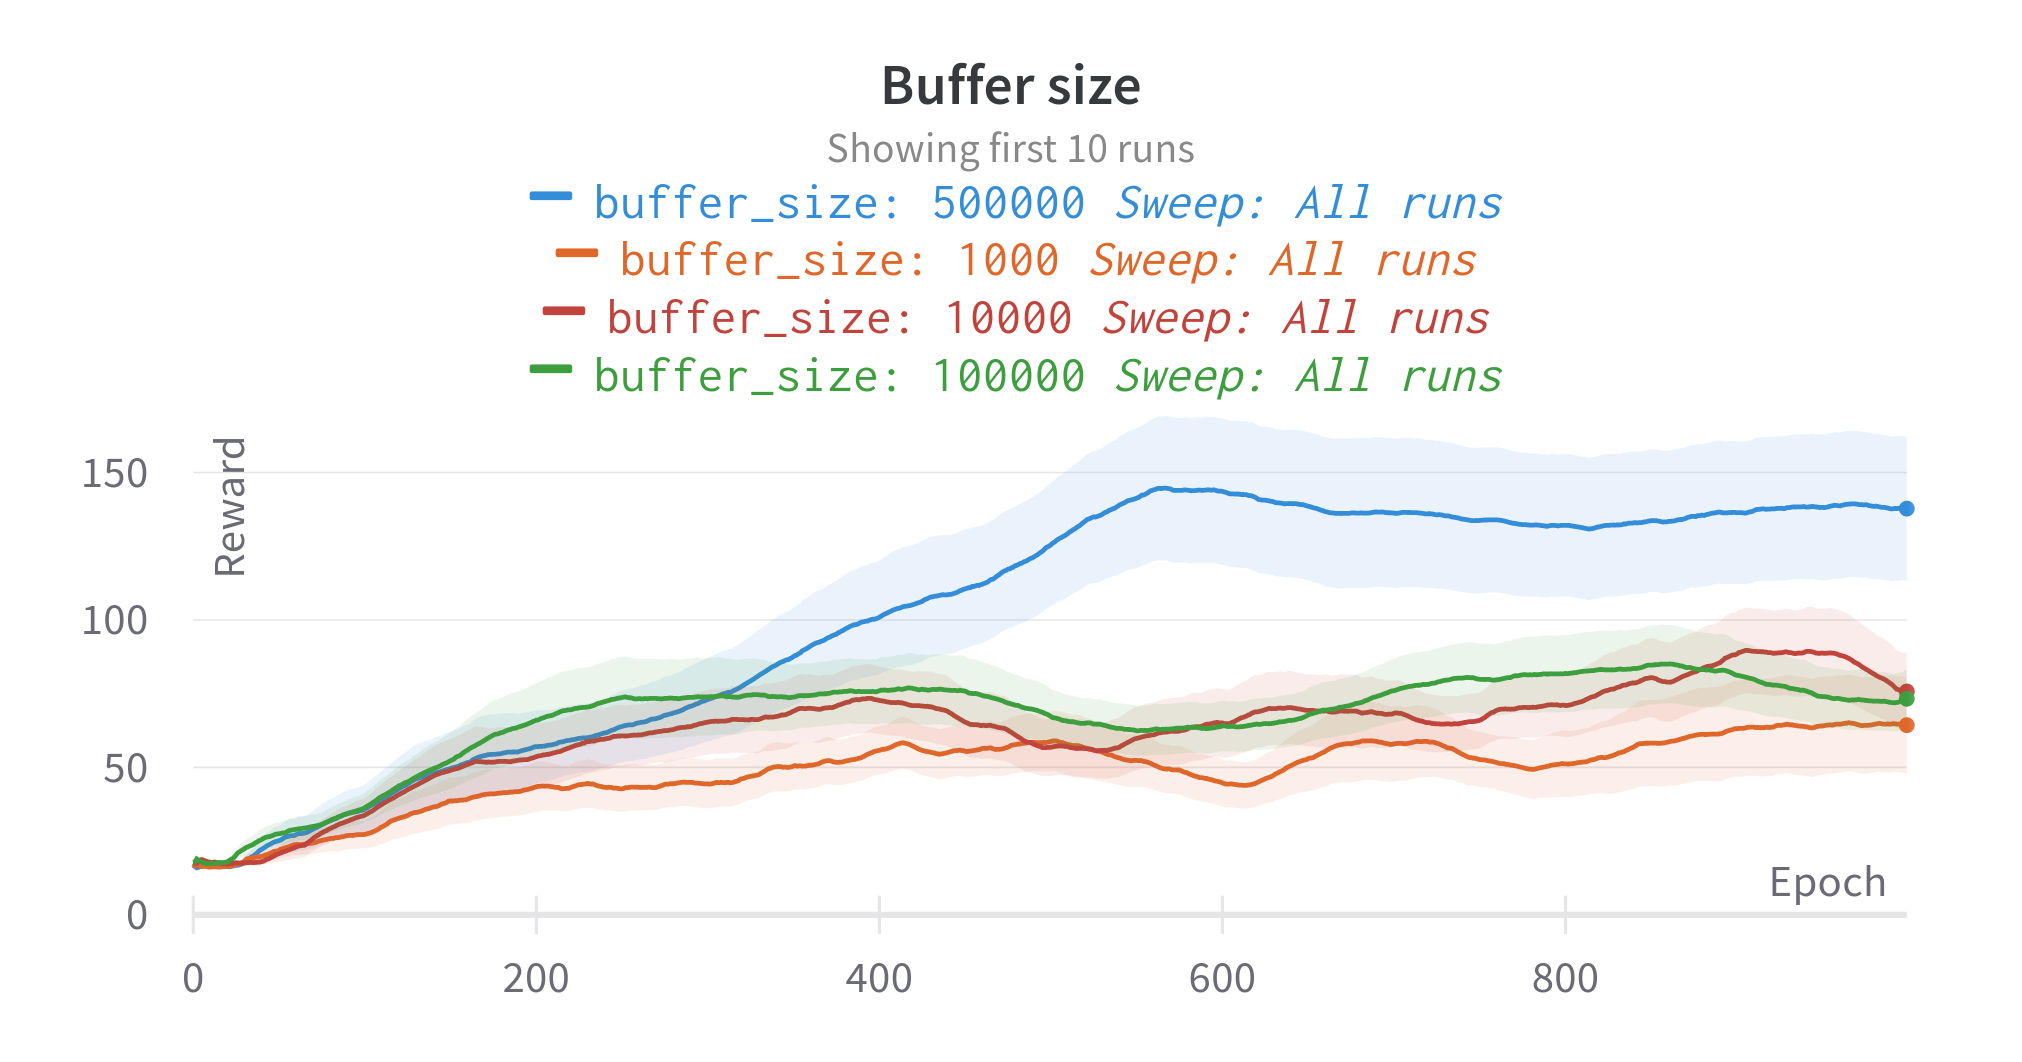
\includegraphics[width=\columnwidth]{assets/hyperparamter-scan/W&B Chart Buffer size.png}
   \caption{The influence of the experience buffer size on the average reward of the last 100 epochs is shown. The values are based on the runs from the hyperparameter scan.
   }
   \label{fig_hyperparameter_scan_isolated_buffer_size}
\end{figure}

\section{Team member contributions}
Andrija implemented the DQN with ER and TN, experiment configs and executed experiments. % TODO
Tom implemented plotting, improved the DQN implementation, executed experiments and did the hyperparameter scan with Weights and Biases.
Tommaso configured the experiments. % TODO
The report was written with equal contribution from everyone.


\end{document}


% This document was modified from the file originally made available by
% Pat Langley and Andrea Danyluk for ICML-2K. This version was created
% by Iain Murray in 2018, and modified by Alexandre Bouchard in
% 2019 and 2021. Previous contributors include Dan Roy, Lise Getoor and Tobias
% Scheffer, which was slightly modified from the 2010 version by
% Thorsten Joachims & Johannes Fuernkranz, slightly modified from the
% 2009 version by Kiri Wagstaff and Sam Roweis's 2008 version, which is
% slightly modified from Prasad Tadepalli's 2007 version which is a
% lightly changed version of the previous year's version by Andrew
% Moore, which was in turn edited from those of Kristian Kersting and
% Codrina Lauth. Alex Smola contributed to the algorithmic style files.
